\documentclass[12pt]{article}
\usepackage[utf8]{inputenc}
\usepackage{geometry}
\usepackage{SIunits}
\usepackage{graphicx}
\usepackage{booktabs}
\usepackage{listings}
\usepackage{color}
\usepackage{placeins}
\usepackage{rotating}
\usepackage{fullpage}

\definecolor{mygreen}{rgb}{0, 0.25, 0}

\lstset{
    tabsize = 2,
    breaklines = true,
    commentstyle = \color{mygreen} \bfseries,
    keywordstyle = \color{blue}  \bfseries,
    frame = single,
    numberstyle = \color{red}  \bfseries,
    captionpos = b,
    basicstyle = \ttfamily,
    language = verilog
}

\begin{document}

\begin{titlepage}
    \center
    \qquad\\[7cm]
    \textsc{\huge \bfseries Laboratory Exercise B} \\[.5cm]
    \textsc{\huge \bfseries Counters} \\[1.0cm]
    {\large TCES330 Digital Systems Design} \\[.5cm]
    {\large Spring 2014} \\[1.5cm]
    
    \begin{tabular}{ll}
        \multicolumn{2}{l}{\textbf{Authors:}}   \\
        Chad Condon:        & \underline{\hspace{5cm}} \\
        Brian Crabtree:     & \underline{\hspace{5cm}} \\
        Ben Foster:         & \underline{\hspace{5cm}} \\
        Aaron Stephens:     & \underline{\hspace{5cm}} \\
        Submission Data:    & June 6, 2014
    \end{tabular}
    
\end{titlepage}

\tableofcontents
\pagebreak

\section*{Laboratory Assignment 2} \addcontentsline{toc}{section}{Laboratory Assignment 2}

\section{Requirements} \label{sec:requirements}

\begin{itemize}
    \item Implement the six-instruction programmable processor described in
    \href{https://moodle.insttech.washington.edu/mod/resource/view.php?id=32929}{Lecture 16b} using Verilog.
    \item Your Quartus project should be in a folder called \verb|LabB| and your top-level module should be called \verb|LabB|.
    Your top-level module will instantiate your processor module and interface to the DE2 board as follows:
    \begin{itemize}
        \item \verb|KEY[0]| acts as your system clock.
        \item \verb|KEY[1]| acts as a synchronous system reset.\footnote{%
            Note that reset will not be able reload memory contents,
            but it should reinitialize your state machine and reset (clear) \underline{all} your registers.
        }
        \item Several internal variables are brought to the top-level for debug and display purposes.
        These include the program counter, the instruction register, state machine current state,
        both inputs to the ALU, the ALU output, the contents of Register File 0, the output of the datapath multiplexer.
        \item \verb|HEX3|, \verb|2|, \verb|1|, and \verb|0| displays the current contents of the IR.
        \item \verb|SW[17:15]| determines what \verb|HEX7|, \verb|6|, \verb|5|, and \verb|4| display as follows:
        \begin{itemize}
            \item 0: \verb|HEX7| = 0; \verb|HEX6|, \verb|HEX5| = PC; \verb|HEX4| = Current State;
            \item 1: \verb|HEX7|, \verb|6|, \verb|5|, \verb|4| = ALU\_A (A-side input to ALU)
            \item 2: \verb|HEX7|, \verb|6|, \verb|5|, \verb|4| = ALU\_B (B-side input to ALU)
            \item 3: \verb|HEX7|, \verb|6|, \verb|5|, \verb|4| = ALU\_Out (ALU output)
            \item 4: Unused (use this for your own debug information)
            \item 5: \verb|HEX7|, \verb|6|, \verb|5|, \verb|4| = Register File 0 contents
            \item 6: \verb|HEX7|, \verb|6|, \verb|5|, \verb|4| = Datapath Multiplexer output
            \item 7: Unused (use this for your own debug information)
        \end{itemize}
    \end{itemize}
    \item A suggested signature for your Processor module:
    \begin{lstlisting}
module Processor( Clk, Reset, IR_Out, PC_Out, StateO, ALU_A, ALU_B, ALU_Out, RQ0, Mux_out);
    input Clk;              // system clock
    input Reset;            // system reset
    output [15:0] IR_Out;   // Instruction register
    output [4:0] PC_Out;    // Program counter
    output [3:0] StateO;    // FSM current state
    output [15:0] ALU_A;    // ALU A-Side Input
    output [15:0] ALU_B;    // ALU B-Side Input
    output [15:0] ALU_Out;  // ALU current output
    output [15:0] RQ0;      // RF[0] contents
    output [15:0] Mux_out;  // Datapath mux output
    \end{lstlisting}
    Feel free to add debug outputs to your processor module.
    \item Turn in the following sample program compiled and loaded into Instruction Memory:
    \begin{lstlisting}
RF[0] = D[A] - D[1A] + D[3] - D[8A];
D[BB] = RF[0];
HALT
    \end{lstlisting}
    Data memory should contain:
    \begin{lstlisting}
D[3] = 0x10AA
D[A] = 0xB0C5
D[1A] = 0x00DC
D[8A] = 0x00E9
    \end{lstlisting}
    \item Make sure that the In System Memory Content Editor can display the contents of both of your memories.
    \item Make sure Quartus recognizes your state machine (as a state machine).
    \item Data memory should be a $256 \times 16$ Quartus RAM LPM with Memory Content Editor enabled.
    \item The Register File should be from Homework 6.
    \item The ALU should be from Homework 6.
    \item The Instruction memory should be a $32 \times  16$ Quartus ROM LPM with Memory Content Editor enabled.
    \item The controller state machine should be similar to the one shown in Lecture 16b.
    \item Implement a ModelSim testbench project that exercises your processor with the required program.
    You may wish to test with additional programs,
    but the \verb|*.mif| files you turn in should contain the instructions
    and data necessary to implement the program shown above.
    \item Write your report using the same outline as before.
    You know by now to be very explicit and detailed about your test procedure and test results.
    Photographs are allowed.
\end{itemize} \FloatBarrier \clearpage

\section{Design} \label{sec:design}

Analysis of the requirements described in \hyperref[sec:requirements]{Section \ref*{sec:requirements} } as well as those in \href{https://moodle.insttech.washington.edu/mod/resource/view.php?id=32929}{Lecture 16b} yielded the hierarchy shown in \hyperref[fig:hierarchy]{Figure \ref*{fig:hierarchy}}.
The design of each module will be discussed below.

\begin{figure}[htbp]
    \centering
    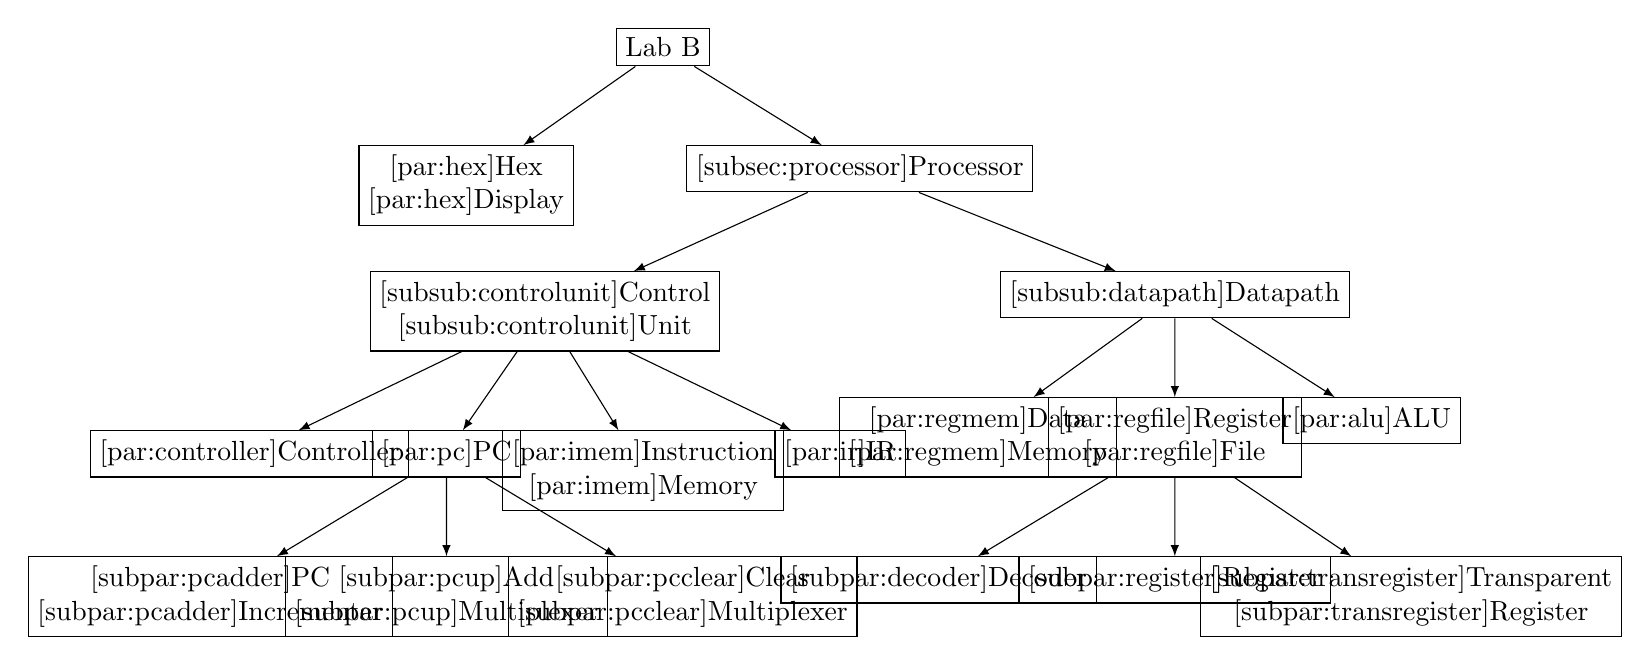
\begin{tikzpicture}[
            every node/.style={rectangle, align=center},
            level/.style={growth parent anchor=south, level distance=1cm},
            level 1/.style={sibling distance=5cm},
            level 2/.style={sibling distance=8cm},
            level 3/.style={sibling distance=2.5cm},
            level 4/.style={sibling distance=3cm},
            edge from parent/.style={draw,-latex},
            every child node/.style={anchor=north}]
        \node [draw] (top) {Lab B}
            child {node [draw] (Hex7Seg) {\hyperref[par:hex]{Hex}\\\hyperref[par:hex]{Display}}}
            child {node [draw] (Processor) {\hyperref[subsec:processor]{Processor}}
                child {node [draw] (cunit) {\hyperref[subsub:controlunit]{Control}\\\hyperref[subsub:controlunit]{Unit}}
                    child {node [draw] (controller) {\hyperref[par:controller]{Controller}}}
                    child {node [draw] (PC) {\hyperref[par:pc]{PC}}
                        child {node [draw] (PCAdderer) {\hyperref[subpar:pcadder]{PC}\\\hyperref[subpar:pcadder]{Incrementer}}}
                        child {node [draw] (PCUp) {\hyperref[subpar:pcup]{Add}\\\hyperref[subpar:pcup]{Multiplexer}}}
                        child {node [draw] (PCClear) {\hyperref[subpar:pcclear]{Clear}\\\hyperref[subpar:pcclear]{Multiplexer}}}
                    }
                    child {node [draw] (imemlpm) {\hyperref[par:imem]{Instruction}\\\hyperref[par:imem]{Memory}}}
                    child {node [draw] (IR) {\hyperref[par:ir]{IR}}}
                }
                child {node [draw] (Datapath) {\hyperref[subsub:datapath]{Datapath}}
                    child {node [draw] (RAM) {\hyperref[par:regmem]{Data}\\\hyperref[par:regmem]{Memory}}}
                    child {node [draw] (RegisterFile) {\hyperref[par:regfile]{Register}\\\hyperref[par:regfile]{File}}
                    child {node [draw] (PCClear) {\hyperref[subpar:decoder]{Decoder}}}
                        child {node [draw] (PCClear) {\hyperref[subpar:register]{Register}}}
                        child {node [draw] (PCClear) {\hyperref[subpar:transregister]{Transparent}\\\hyperref[subpar:transregister]{Register}}}
                    }
                    child {node [draw] (ALU) {\hyperref[par:alu]{ALU}}}
                }
            };
    \end{tikzpicture}
    \caption{Design Hierachy \label{fig:hierarchy}}
\end{figure}

The top-level module must have the properties listed below.

\begin{itemize}
    \item One one-bit input $KEY_0$ as the clock signal.
    \item One one-bit input $KEY_1$ as the active low reset signal.
    \item One two-bit input $SW_{17:15}$ as the display select signal.
    \item Four seven-bit outputs $HEX0$, $HEX1$, $HEX2$, and $HEX3$ as the instruction display.
    \item Four seven-bit outputs $HEX4$, $HEX5$, $HEX6$, and $HEX7$ as selectable display.
    \item The value of $SW_{17:15}$ selects the value to be displayed on $HEX4$, $HEX5$, $HEX6$, and $HEX7$ as shown in \hyperref[tab:display]{Table \ref*{tab:display}}.
\end{itemize}

\begin{table}[htbp] 
    \centering
    \begin{tabular}{ll}                             \toprule
        $SW_{17:15}$    & Displayed Values              \\\midrule
        0               & Current State                 \\
        1               & A side input to ALU           \\
        2               & B side input to ALU           \\
        3               & ALU output                    \\
        4               & \emph{Unused}                 \\
        5               & Register File 0 contents      \\
        6               & Datapath multiplexer output   \\
        7               & \emph{Unused}                 \\\bottomrule
    \end{tabular}
\caption{Selectable Display Values\label{tab:display}}
\end{table}

The file \verb|LabB.v| contains the module \verb|LabB| which satisfies these properties.
A listing can be found in the \hyperref[sec:appendix]{Appendix}, \hyperref[lst:LabB]{Listing \ref*{lst:LabB}}.

\paragraph{Hex Display} \label{par:hex}

The top-level module required a hex display Verilog module with the properties listed below.
This module was reused from Homework 2.

\begin{itemize}
    \item One four-bit input $C$ as the displayed value.
    \item One seven-bit output $Display$ as the seven segment display.
    \item Assigns $Display$ to the appropriate value to display the hexadecimal character representing $C$'s value on a seven segment display.
\end{itemize}

The file \verb|Hex7seg.v| contains the module \verb|Hex7seg| which satisfies these properties.
A listing can be found in the \hyperref[sec:appendix]{Appendix}, \hyperref[lst:hex]{Listing \ref*{lst:hex}}.

\subsection{Processor}  \label{subsec:processor}

The top-level module required a processesor Verilog modules with the properties listed below.

\begin{itemize}
    \item One one-bit input $Clk$ as the clock signal.
    \item One one-bit input $Reset$ as the active high reset signal.
    \item One sixteen-bit output $IR_\text{Out}$ as the instruction register value.
    \item One five-bit output $PC_\text{Out}$ as the program counter value.
    \item One four-bit output $State0$ as the current state.
    \item Two sixteen-bit outputs $ALU_A$ and $ALU_B$ as the A- and B-side ALU inputs respectively.
    \item One sixteen-bit output $ALU_\text{Out}$ as the ALU output.
    \item One sixteen-bit output $RQ0$ as the register file 0 entry.
    \item One sixteen-bit output $Mux_\text{out}$ as the datapath multiplexer output.
\end{itemize}

The file \verb|Processor.v| contains the module \verb|Processor| which satisfies these properties.
A listing can be found in the \hyperref[sec:appendix]{Appendix}, \hyperref[lst:processor]{Listing \ref*{lst:processor}}.

\subsubsection{Control Unit} \label{subsub:controlunit}

The processor module required a control unit Verilog module with the properties listed below.

\begin{itemize}
    \item One one-bit input $Clock$ as the clock signal.
    \item One eight-bit output $D_text{addr}$ as the data memory address.
    \item One four-bit output $RF_{W_\text{addr}}$ as the register file write address.
    \item Two four-bit outputs $RF_{Ra_\text{addr}}$ and $RF_{Rab_\text{addr}}$ as the register file A and B stream read addresses respectively.
    \item One one-bit output $D_\text{wr}$ as the data memory write enable signal.
    \item One one-bit output $RF_s$ as the data multiplexer select signal.
    \item One three-bit output $Alu_{s0}$ as the ALU function select signal.
    \item One one-bit output $RF_{W_\text{wr}}$ as the register file write enable signal.
    \item Two one-bit inputs $RF_{Ra_\text{rd}}$ and $RF_{Rab_\text{rd}}$ as the register file A and B stream read enable signals respectively.
    \item One One five-bit output $RC_\text{Out}$ as the program counter address.
    \item One sixteen-bit output $IR_\text{Out}$ as the current instruction.
    \item One four-bit output $State0$ as the controller state. 
\end{itemize}

The file \verb|cunit.v| contains the module \verb|cunit| which satisfies these properties.
A listing can be found in the \hyperref[sec:appendix]{Appendix}, \hyperref[lst:cunit]{Listing \ref*{lst:cunit}}.

\paragraph{Program Counter} \label{par:pc}

The control unit module required a program counter Verilog module with the properties listed below.

\begin{itemize}
    \item One one-bit input $Clear$ as the active high, synchronous clear signal.
    \item One one-bit input $Up$ as the load enable signal.
    \item One one-bit input $Clock$ as the clock signal.
    \item One five-bit output $O$ as the program counter value.
\end{itemize}

The file \verb|PC.v| contains the module \verb|PC| which satisfies these properties.
A listing can be found in the \hyperref[sec:appendix]{Appendix}, \hyperref[lst:pc]{Listing \ref*{lst:pc}}.

\subparagraph{PC Incrementer} \label{subpar:pcadder}

The program counter module required a PC incrementer Verilog module with the properties listed below.

\begin{itemize}
    \item One five-bit input $I$.
    \item One five-bit output $O$ which passes the sum $I + 1$.
\end{itemize}

The file \verb|PCAdder.v| contains the module \verb|PCAdder| which satisfies these properties.
A listing can be found in the \hyperref[sec:appendix]{Appendix}, \hyperref[lst:PCAdder]{Listing \ref*{lst:PCAdder}}.

\subparagraph{Add Multiplexer} \label{subpar:pcup}

The program counter module required an add multiplexer Verilog module with the properties listed below.

\begin{itemize}
    \item Two one-bit inputs $data0x$ and $data1x$ as the selectable inputs.
    \item One one-bit input $sel$ as the select signal.
    \item One one-bit output $result$ which passes $data0x$ or $data1x$ if $sel$ is 0 or 1 respectively.
\end{itemize}


The file \verb|PCUp.v| contains the module \verb|PCUp| which satisfies these properties from the Altera library of parameterized modules.
A listing can be found in the \hyperref[sec:appendix]{Appendix}, \hyperref[lst:PCUp]{Listing \ref*{lst:PCUp}}.

\subparagraph{Clear Multiplexer} \label{subpar:pcclear}

The program counter module required a clear multiplexer Verilog module with the properties listed below.

\begin{itemize}
    \item Two one-bit inputs $data0x$ and $data1x$ as the selectable inputs.
    \item One one-bit input $sel$ as the select signal.
    \item One one-bit output $result$ which passes $data0x$ or $data1x$ if $sel$ is 0 or 1 respectively.
\end{itemize}

The file \verb|PCClear.v| contains the module \verb|PCClear| which satisfies these properties from the Altera library of parameterized modules.
A listing can be found in the \hyperref[sec:appendix]{Appendix}, \hyperref[lst:PCClear]{Listing \ref*{lst:PCClear}}.

\paragraph{Instruction Register} \label{par:ir}

The control unit module required an instruction register Verilog module with the properties listed below.

\begin{itemize}
    \item Parameterized data bit width $N$.
    \item One one-bit input $clk$ as the clock signal.
    \item One $N$-bit input $d$ as the input value.
    \item One one-bit input $ir_\text{ld}$ as the load enable signal.
    \item One $N$-bit output $q$ as the register's value.
\end{itemize}

The file \verb|instruction_register.v| contains the module \verb|instruction_register| which satisfies these properties.
A listing can be found in the \hyperref[sec:appendix]{Appendix}, \hyperref[lst:ir]{Listing \ref*{lst:ir}}.

\paragraph{Controller} \label{par:controller}

The control unit module required controller Verilog module with the properties listed below.

\begin{itemize}
    \item One sixteen-bit input $instruction$ which accepts an intruction.
    \item One one-bit input $clk$ which acts as the clock.
    \item One one-bit output $PC_\text{clr}$ which signals to clear the program counter.
    \item One one-bit output $PC_\text{up}$ which signals to increment to program counter.
    \item One one-bit output $IR_\text{ld}$ which signals to load the instruction register.
    \item One one-bit output $RF_\text{s}$ which selects the register file.
    \item One one-bit output $RF_{W_\text{wr}}$ which signals to write enable the register file.
    \item One one-bit output $RF_{Ra_\text{rd}}$ which signals to read enable the A stream of the register file.
    \item One one-bit output $RF_{Rb_\text{rd}}$ which signals to read enable the B stream of the regoster file.
    \item One eight-bit output $D_\text{addr}$ which signals the data memory address.
    \item One one-bit output $D_wr$ which signals to write enable the data memory.
    \item One four-bit output $RF_{W_\text{addr}}$ which signals the register file's write address.
    \item One four-bit output $RF_{Ra_\text{addr}}$ which signals the register file's A stream read address.
    \item One four-bit output $RF_{Rb_\text{addr}}$ which signals the register files' B stream read address.
    \item One four-bit output $Alu_\text{s0}$ which selects the arithmetic logic unit's function.
    \item One four-bit output $State$ which signals the current state,
    \item Positive edge triggered.
    \item Quartus recognized state machine.
    \item Ten states representing each phase of each instruction.\footnote{See \hyperref[tab:instructions]{Table \ref*{tab:instructions}} for a list of instructions.}
    \begin{itemize}
        \item \textbf{INIT}: Wait
        \item \textbf{FETCH}: Retrieve new instruction
        \item \textbf{DECODE}: Interpret instruction
        \item \textbf{NOOP}: Do nothing
        \item \textbf{LOAD\_A}: Begin load operation
        \item \textbf{LOAD\_B}: Complete load operation
        \item \textbf{STORE}: Store operation
        \item \textbf{ADD}: Addition operation
        \item \textbf{SUB}: Substraction operation
        \item \textbf{HALT}: Stop all operations
    \end{itemize}
\end{itemize}

The file \verb|controller.v| contains the module \verb|controller| which satisfies these properties.
A listing can be found in the \hyperref[sec:appendix]{Appendix}, \hyperref[lst:controller]{Listing \ref*{lst:controller}}.

\paragraph{Instruction Memory} \label{par:imem}

The control unit module required an instruction memory Verilog module with the properties listed below.

\begin{itemize}
    \item One five-bit input $address$ as the data address.
    \item One one-bit input $clock$ as the clock signal.
    \item One sixteen-bit output $q$ as the data read signal.
\end{itemize}

The file \verb|imemlpm.v| contains the module \verb|imemlpm| which satisfies these properties from the Altera library of parameterized modules.
A listing can be found in the \hyperref[sec:appendix]{Appendix}, \hyperref[lst:imemlpm]{Listing \ref*{lst:imemlpm}}.

\subsubsection{Datapath} \label{subsub:datapath}

The processor module required datapath Verilog module with the properties listed below.

\begin{itemize}
    \item One one-bit input $Clock$ as the clock signal.
    \item One one-bit input $Reset$ as an active high, synchronous reset signal.
    \item One eight-bit input $D_\text{addr}$ as the data memory address.
    \item One one-bit input $D_\text{wr}$ as the data memory write enable signal.
    \item One four-bit input $RF_{W_\text{addr}}$ as the register file write address.
    \item One one-bit input $RF_{W_\text{wr}}$ as the register file write enable signal.
    \item One four-bit input $RF_{Ra_\text{addr}}$ as the register file stream A read address.
    \item One one-bit input $RF_{Ra_\text{rd}}$ as the register file stream A read enable signal.
    \item One four-bit input $RF_{Rb_\text{addr}}$ as the register file stream B read address.
    \item One one-bit input $RF_{Rb_\text{rd}}$ as the register file stream B read enable signal.
    \item One three-bit input $Alu_{s0}$ as the ALU function select signal.
    \item Two sixteen-bit outputs $ALU_A$ and $ALU_B$ as the ALU A- and B-side inputs respectively.
    \item One sixteen-bit output $RQ0$ as the first register file entry.
    \item One sixteen-bit output $Mux_\text{out}$ as register file write data input.
    \item Positive edge triggered.
\end{itemize}

The file \verb|Datapath.v| contains the module \verb|Datapath| which satisfies these properties.
A listing can be found in the \hyperref[sec:appendix]{Appendix}, \hyperref[lst:datapath]{Listing \ref*{lst:datapath}}.

\paragraph{Data Memory} \label{par:regmem}

The datapath module required register memory Verilog module with the properties listed below.
This module was reused frome Homework 6.

\begin{itemize}
    \item One eight-bit input $address$ as the read/write address.
    \item One one-bit input $clock$ as the clock signal.
    \item One sixteen-bit input $data$ as the data to write.
    \item One one-bit input $wren$ as the write-enable signal.
    \item One sixteen-bit output $q$ as the read data stream.
    \item Positive edge-triggered.
    \item $256 \times 16$ Quartus RAM LPM with Memory Content Editor enabled.
\end{itemize}

The file \verb|ramlpm.v| contains the module \verb|ramlpm| which satisfies these properties from the Altera library of parameterized modules.
A listing can be found in the \hyperref[sec:appendix]{Appendix}, \hyperref[lst:ramlpm]{Listing \ref*{lst:ramlpm}}.

\paragraph{Register File} \label{par:regfile}

The datapath module required a register file Verilog module with the properties listed below.
This module was reused from Homework 6.

\begin{itemize}
    \item One one-bit input $Clk$ as the clock signal.
    \item One one-bit input $Reset$ as an active high reset signal.
    \item One sixteen-bit input $W_\text{data}$ as the data to write.
    \item One four-bit input $W_\text{addr}$ as the write address.
    \item One one-bit input $W_\text{en}$ as the write enable signal.
    \item Two four-bit inputs $R_\text{addr0}$ and $R_\text{addr1}$ as the A and B stream read addresses respectively.
    \item Two one-bit inputs $R_\text{en0}$ and $R_\text{en1}$ as the A and B stream read enable signals respectively.
    \item Two sixteen-bit outputs $R_\text{data0}$ and $R_\text{data1}$ as the A and B data streams respectively.
    \item One sixteen-bit output $RQ0$ which signals the contents of register 0.
    \item Positive edge triggered.
\end{itemize}

The file \verb|RegisterFile.v| contains the module \verb|RegisterFile| which satisfies these properties.
A listing can be found in the \hyperref[sec:appendix]{Appendix}, \hyperref[lst:registerfile]{Listing \ref*{lst:registerfile}}.

\subparagraph{Decoder} \label{subpar:decoder}

The register file module required a decoder Verilog module with the properties listed below.
This module was reused from Homework 6.

\begin{itemize}
    \item Parameterized input size $N$.
    \item One $N$-bit select input $W$.
    \item One one-bit enable input $E$.
    \item One $2^N$-bit output $Y$.
    \item ``One hot'' decoder with enable.
\end{itemize}

The file \verb|DecoderN.v| contains the module \verb|DecoderN| which satisfies these properties.
A listing can be found in the \hyperref[sec:appendix]{Appendix}, \hyperref[lst:DecoderN]{Listing \ref*{lst:DecoderN}}.

\subparagraph{Register} \label{subpar:register}

The register file module required a register Verilog module with the properties listed below.
This module was reused from Homework 6.

\begin{itemize}
    \item Paramerized data size $N$
    \item One one-bit input $Clk$ which acts as the clock.
    \item One one-bit input $Rst$ which acts as an active high reset.
    \item One one-bit input $Ld$ which acts as a load enable.
    \item One one-bit input $Oe0$ which acts as the A stream output enable.
    \item One one-bit input $Oe1$ which acts as the B stream output enable.
    \item One $N$-bit input $I$ which acts as the data to load.
    \item One $N$-bit output $Qz0$ which acts as the A stream switched output.
    \item One $N$-bit output $Qz1$ which acts as the B stream switched output.
    \item Positive edge triggered.
    \item Holds the value of $I$ when $Ld = 1$.
    \item Outputs the data to $Qz0$ and $Qz1$ when $Oe0$ and $Oe1$ are high respectively.
    \item Outputs high impedence otherwise.
\end{itemize}

The file \verb|RegisterOEN.v| contains the module \verb|RegisterOEN| which satisfies these properties.
A listing can be found in the \hyperref[sec:appendix]{Appendix}, \hyperref[lst:RegisterOEN]{Listing \ref*{lst:RegisterOEN}}.

\subparagraph{Transparent Register} \label{subpar:transregister}

The register file moduule required a transparent register Verilog module witht he properties listed below.

\begin{itemize}
    \item All ports and parameters included from \verb|RegisterOEN| module.
    \item One $N$-bit output $Q_act$ which signals the register's current data.
\end{itemize}

The file \verb|RegisterOENExtraOutput.v| contains the module \verb|RegisterOENExtraOutput| which satisfies these properties.
A listing can be found in the \hyperref[sec:appendix]{Appendix}, \hyperref[lst:RegisterOENExtraOutput]{Listing \ref*{lst:RegisterOENExtraOutput}}.

\paragraph{Arithmetic Logic Unit} \label{par:alu}

The datapath module required an arithmetic logic unit Verilog module with the properties listed below.
This module was reused from Homework 6.

\begin{itemize}
    \item Two sixteen-bit inputs: $A$ and $B$.
    \item One three-bit input: $Sel$.
    \item One sixteen-bit output: $Q$.
    \item $Q$ is a function of $A$ and $B$ as selected by $Sel$ as shown in \hyperref[tab:alu]{Table \ref*{tab:alu}}..
        \begin{table}[htbp]
            \centering
            \begin{tabular}{ll}             \toprule
                $Sel$       & $Q$           \\\midrule
                0           & $0$           \\
                1           & $A + B$       \\
                2           & $A - B$       \\
                3           & $A$           \\
                4           & $A \oplus B$  \\
                5           & $A \lor B$    \\
                6           & $A \land B$   \\
                7           & $A + 1$       \\\bottomrule
            \end{tabular}
            \caption{ALU output}
            \label{tab:alu}
        \end{table}
\end{itemize}

The file \verb|ALU.v| contains the module \verb|ALU| which satisfies these properties.
A listing can be found in the \hyperref[sec:appendix]{Appendix}, \hyperref[lst:alu]{Listing \ref*{lst:alu}}. \FloatBarrier \clearpage

\section{Test Procedures} % (fold)
\label{sec:test_procedures}

The following test procedures will be used to verify that each part of this laboratory exercise satisfies the requirements given in \hyperref[sec:requirements]{Section \ref*{sec:requirements}}.

\subsection{PC Incrementer} % (fold)
\label{sub:pc_incrementer}

% subsection pc_incrementer (end)

\subsection{Add Multiplexer} % (fold)
\label{sub:add_multiplexer}

The add multiplexer module, \verb|PCUp|, was a simple LPM module and will therefore not be specifically tested.
% subsection add_multiplexer (end)

\subsection{Clear Multiplexer} % (fold)
\label{sub:clear_multiplexer}

The clear multiplexer module, \verb|PCClear|, was a simple LPM module and will therefore not be specifically tested.
% subsection clear_multiplexer (end)

\subsection{Decoder} % (fold)
\label{sub:decoder}

The decoder module, \verb|DecoderN|, has been previously used and tested for Homework 6 and will therefore not be specifically tested.
% subsection decoder (end)

\subsection{Register} % (fold)
\label{sub:register}

The register module, \verb|RegisterOEN|, has been previously used and tested for Homework 6  and only minimally modified.
It will therefore not be specifically tested.
% subsection register (end)

\subsection{Controller} % (fold)
\label{sub:controller}

% subsection controller (end)

\subsection{Program Counter} % (fold)
\label{sub:program_counter}

% subsection program_counter (end)

\subsection{Instruction Memory} % (fold)
\label{sub:instruction_memory}

% subsection instruction_memory (end)


\subsection{Instruction Register} % (fold)
\label{sub:instruction_register}

% subsection instruction_register (end)

\subsection{Data Memory} % (fold)
\label{sub:data_memory}

% subsection data_memory (end)

\subsection{Register File} % (fold)
\label{sub:register_file}

The register file module, \verb|RegisterFile|, has been previously used and tested for Homework 6 and only minimally modified.
It will therefore not be specifically tested.
% subsection register_file (end)

\subsection{Arithmetic Logic Unit} % (fold)
\label{sub:arithmetic_logic_unit}

The arithmetic logic unit module, \verb|ALU|, has been previously used and tested for Homework 6 and will therefore not be specifically tested.
% subsection arithmetic_logic_unit (end)

\subsection{Control Unit} % (fold)
\label{sub:control_unit}

The following test procedure will be used to verify that the Verilog module \verb|cunit| satisfies
the requirements for this part.

%TODO test control unit

% subsection control_unit (end)

\subsection{Datapath} % (fold)
\label{sub:datapath}

The following test procedure will be used to verify that the Verilog module \verb|Datapath| satisfies
the requirements for this part.

%TODO test datapath

% subsection datapath (end)

\subsection{Processor} % (fold)
\label{sub:processor}

The following test procedure will be used to verify that the Verilog module \verb|Processor| satisfies
the requirements for this part.

%TODO test processor

% subsection processor (end)

\subsection{Hex Display} % (fold)
\label{sub:hex_display}

The hex display module, \verb|Hex7seg|, has been previously used and tested for several assignments and will therefore not be specifically tested.
% subsection hex_display (end)

\subsection{Project} % (fold)
\label{sub:project}

The following test procedure will be used to verify that the \emph{Quartus II} project \verb|Lab6| satisfies
the requirements for this lab.

%TODO write up project
\begin{itemize}
    \item The eight instruction processor circuit will be tested using \emph{ModelSim} and the testbench shown in %TODO Figure 9, Appendix A.
    This testbench generates the test vectors shown in \hyperref[tab:project_vectors]{Table \ref*{tab:project_vectors}} and % TODO outputs the multiplexer output M.
    Simulations will be run in order to verify the behavior shown in \hyperref[tab:project_vectors]{Table \ref*{tab:project_vectors}}.
    \item Open the project and verify that compilation produces no errors or unallowed warnings.
    \item Load the project onto the DE2 board without errors.
    \item Generate the test vectors shown in \hyperref[tab:project_vectors]{Table \ref*{tab:project_vectors}} and verify the corresponding outputs,% TODO M.
\end{itemize}

\begin{table}[htbp]
    \centering
    %TODO tabular
    \caption{Project Test Vectors\label{tab:project_vectors}}
\end{table}
% subsection project (end)

% section test_procedures (end) \FloatBarrier \clearpage

\section{Test Results} % (fold)
\label{sec:test_results}

\subsection{PC Incrementer} % (fold)
\label{ssub:pc_incrementer}

% subsection pc_incrementer (end)

\subsection{Controller} % (fold)
\label{ssub:controller}

% subsection controller (end)

\subsection{Program Counter} % (fold)
\label{ssub:program_counter}

% subsection program_counter (end)

\subsection{Instruction Register} % (fold)
\label{ssub:instruction_register}

% subsection instruction_register (end)

\subsection{Control Unit} % (fold)
\label{ssub:control_unit}

% subsection control_unit (end)

\subsection{Datapath} % (fold)
\label{ssub:datapath}

% subsection datapath (end)

\subsection{Processor} % (fold)
\label{ssub:processor}

% subsection processor (end)

\subsection{Project} % (fold)
\label{ssub:projects}

% subsection projects (end)

% section test_results (end) \FloatBarrier \clearpage

\section{Observations} % (fold)
\label{sec:observations}

% section observations (end) \FloatBarrier \clearpage

\subsection*{Conclusion} \addcontentsline{toc}{subsection}{Conclusion}

\clearpage
\FloatBarrier \phantomsection
\addcontentsline{toc}{section}{Appendix}
\section*{Appendix} \label{sec:appendix}

\lstlistoflistings \clearpage

\lstinputlisting[caption = \texttt{LabB.v}, label = lst:LabB]{../LabB.v}
\lstinputlisting[caption = \texttt{Hex7seg.v}, label = lst:hex]{../Hex7seg.v}
\lstinputlisting[caption = \texttt{Processor.v}, label = lst:processor]{../Processor.v}
\lstinputlisting[caption = \texttt{cunit.v}, label = lst:cunit]{../cunit.v}
\lstinputlisting[caption = \texttt{PC.v}, label = lst:pc]{../PC.v}
\lstinputlisting[caption = \texttt{PCAdder.v}, label = lst:PCAdder]{../PCAdder.v}
\lstinputlisting[caption = \texttt{muxlpm.v}, label = lst:muxlpm]{../muxlpm.v}
\lstinputlisting[caption = \texttt{instruction\_register}.v, label = lst:ir]{../instruction_register.v}
\lstinputlisting[caption = \texttt{controller.v}, label = lst:controller]{../controller.v}
\lstinputlisting[caption = \texttt{imemlpm.v}, label = lst:imemlpm]{../imemlpm.v}
\lstinputlisting[caption = \texttt{Datapath.v}, label = lst:datapath]{../Datapath.v}
\lstinputlisting[caption = \texttt{ramlpm.v}, label = lst:ramlpm]{../ramlpm.v}
\lstinputlisting[caption = \texttt{RegisterFile.v}, label = lst:registerfile]{../RegisterFile.v}
\lstinputlisting[caption = \texttt{DecoderN.v}, label = lst:DecoderN]{../DecoderN.v}
\lstinputlisting[caption = \texttt{RegisterOEN.v}, label = lst:RegisterOEN]{../RegisterOEN.v}
\lstinputlisting[caption = \texttt{ALU.v}, label = lst:alu]{../ALU.v}

\end{document}